\chapter{Design}

\section{Transactions}
A peer will have transactions with other peers in the network.
The peer will want to have an increase in his reputation and have a transaction be created.
The transaction contains the information about how much data was uploaded and downloaded between the peers
and their total upload and download amounts.

The transaction will be encapsulated inside a single block.
A block contains both public keys of the peers,
so it is possible to see between which peers the transaction is.
Both peers sign the block to acknowledge that the transaction has happened.
Every block only contains one transaction.

The blocks are linked to previous blocks by adding the hashes of the previous blocks of both peers.
This creates a directed acyclic graph of blocks.
A chain can be identified within this graph for every peer.
This chain contains every transaction of a peer.

An example of three blocks can be seen in Figure \ref{fig:chain-example}.
The arrows denote the corresponding hash or signature.
In this example the first block is between peer B and C.
The block contains hashes to the previous blocks of both B and C
and can be seen by the outward arrows.
Inside the block it can be seen what part peer B and C signs by the boxes.
The whole block is not signed by both parties.
The reason for this is explained in section \ref{design:block_creation}.

In the example both peer B and C also conduct a transaction with another peer, A and D respectively.
This creates two new blocks and are chained to the block between B and C by adding the previous hash to the new blocks.
The new blocks also contains the previous hashes of A and D
and chain the new block to previous blocks of A and D.

\begin{figure}
	\centerline{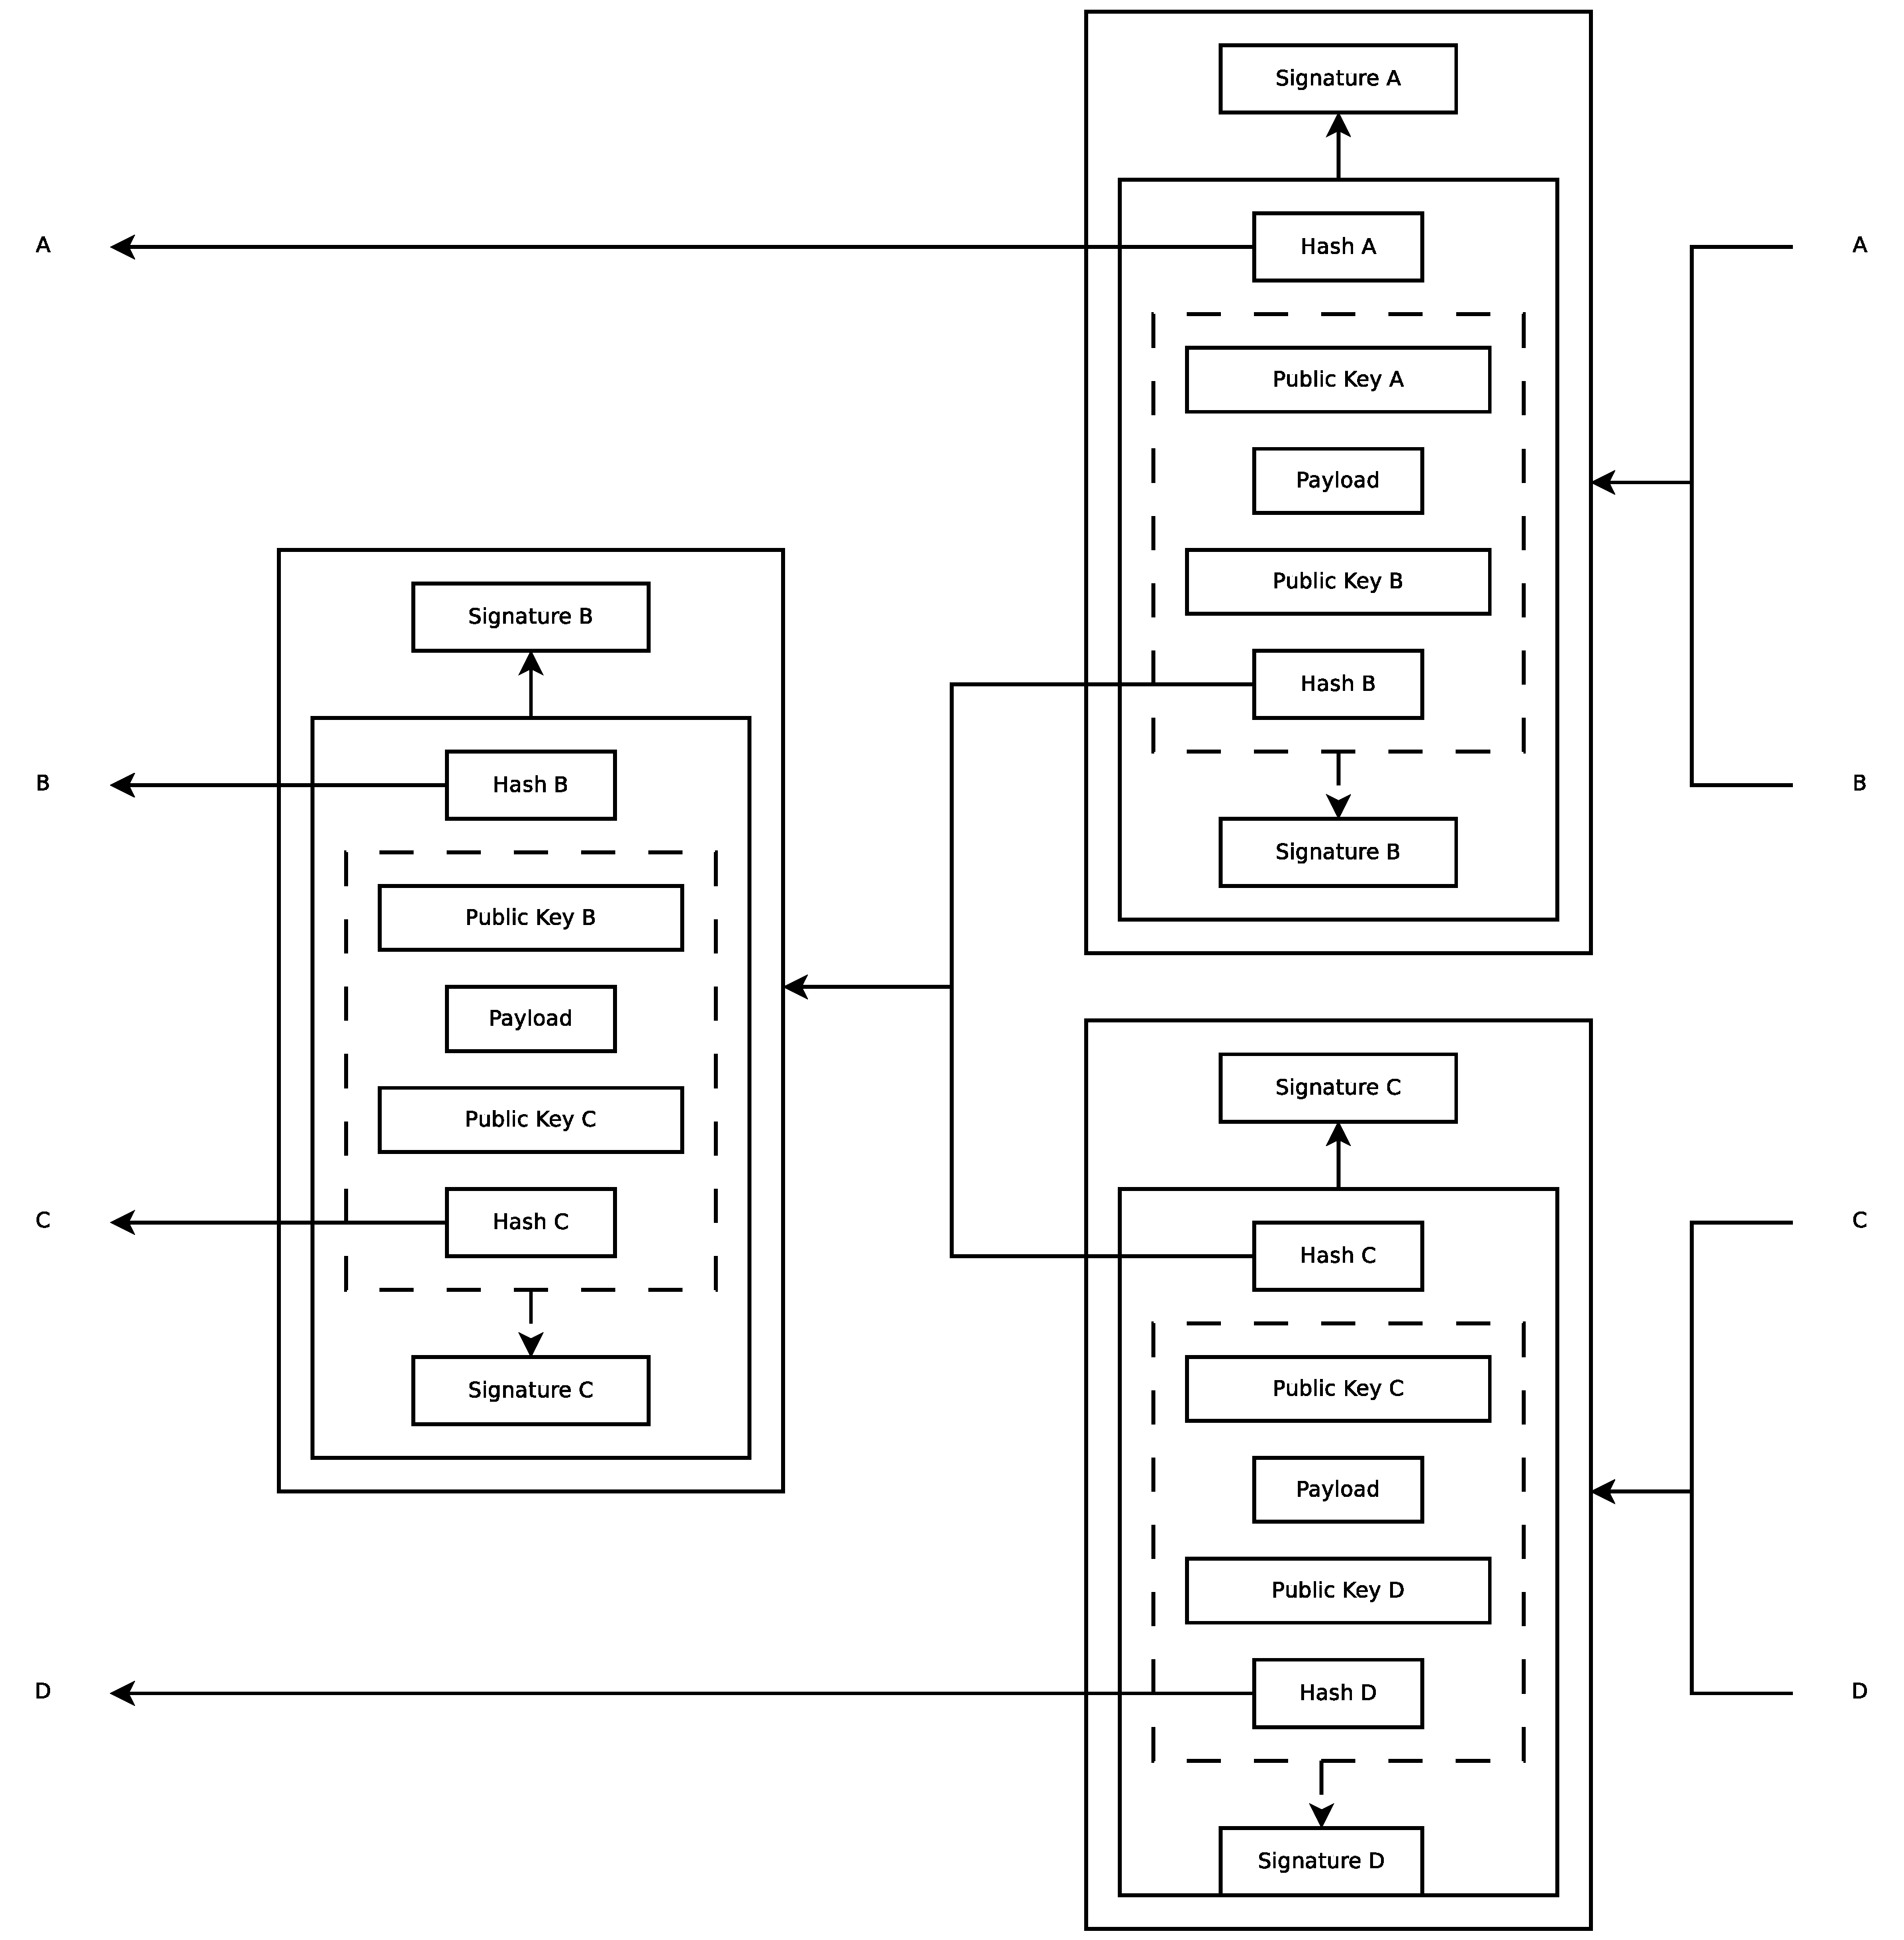
\includegraphics[scale=0.3]{design/figs/chain.eps}}
	\caption{Example of three blocks in the chain.}
	\label{fig:chain-example}
\end{figure}
\subsection{Exchanging signatures}
Two peers in a network will create their blocks together without having to rely on a third party.
Between the peers one is uploading to the other.
The uploader is traditionally called the seeder in BitTorrent and the receiver of this data the downloader\cite{Cohen-bittorrent}.
The seeder will initiate the block creation.\,
co the seeder can decide how altruistic it wants to be towards the downloader regarding its collaboration.
We will explain how the block creation protocol works.
A sequence diagram can be seen in Figure \ref{fig:exchange-new-sequence}.

\begin{figure}[tpb]
\centering
\subfigure[Sequence diagram for block creation]{
\centerline{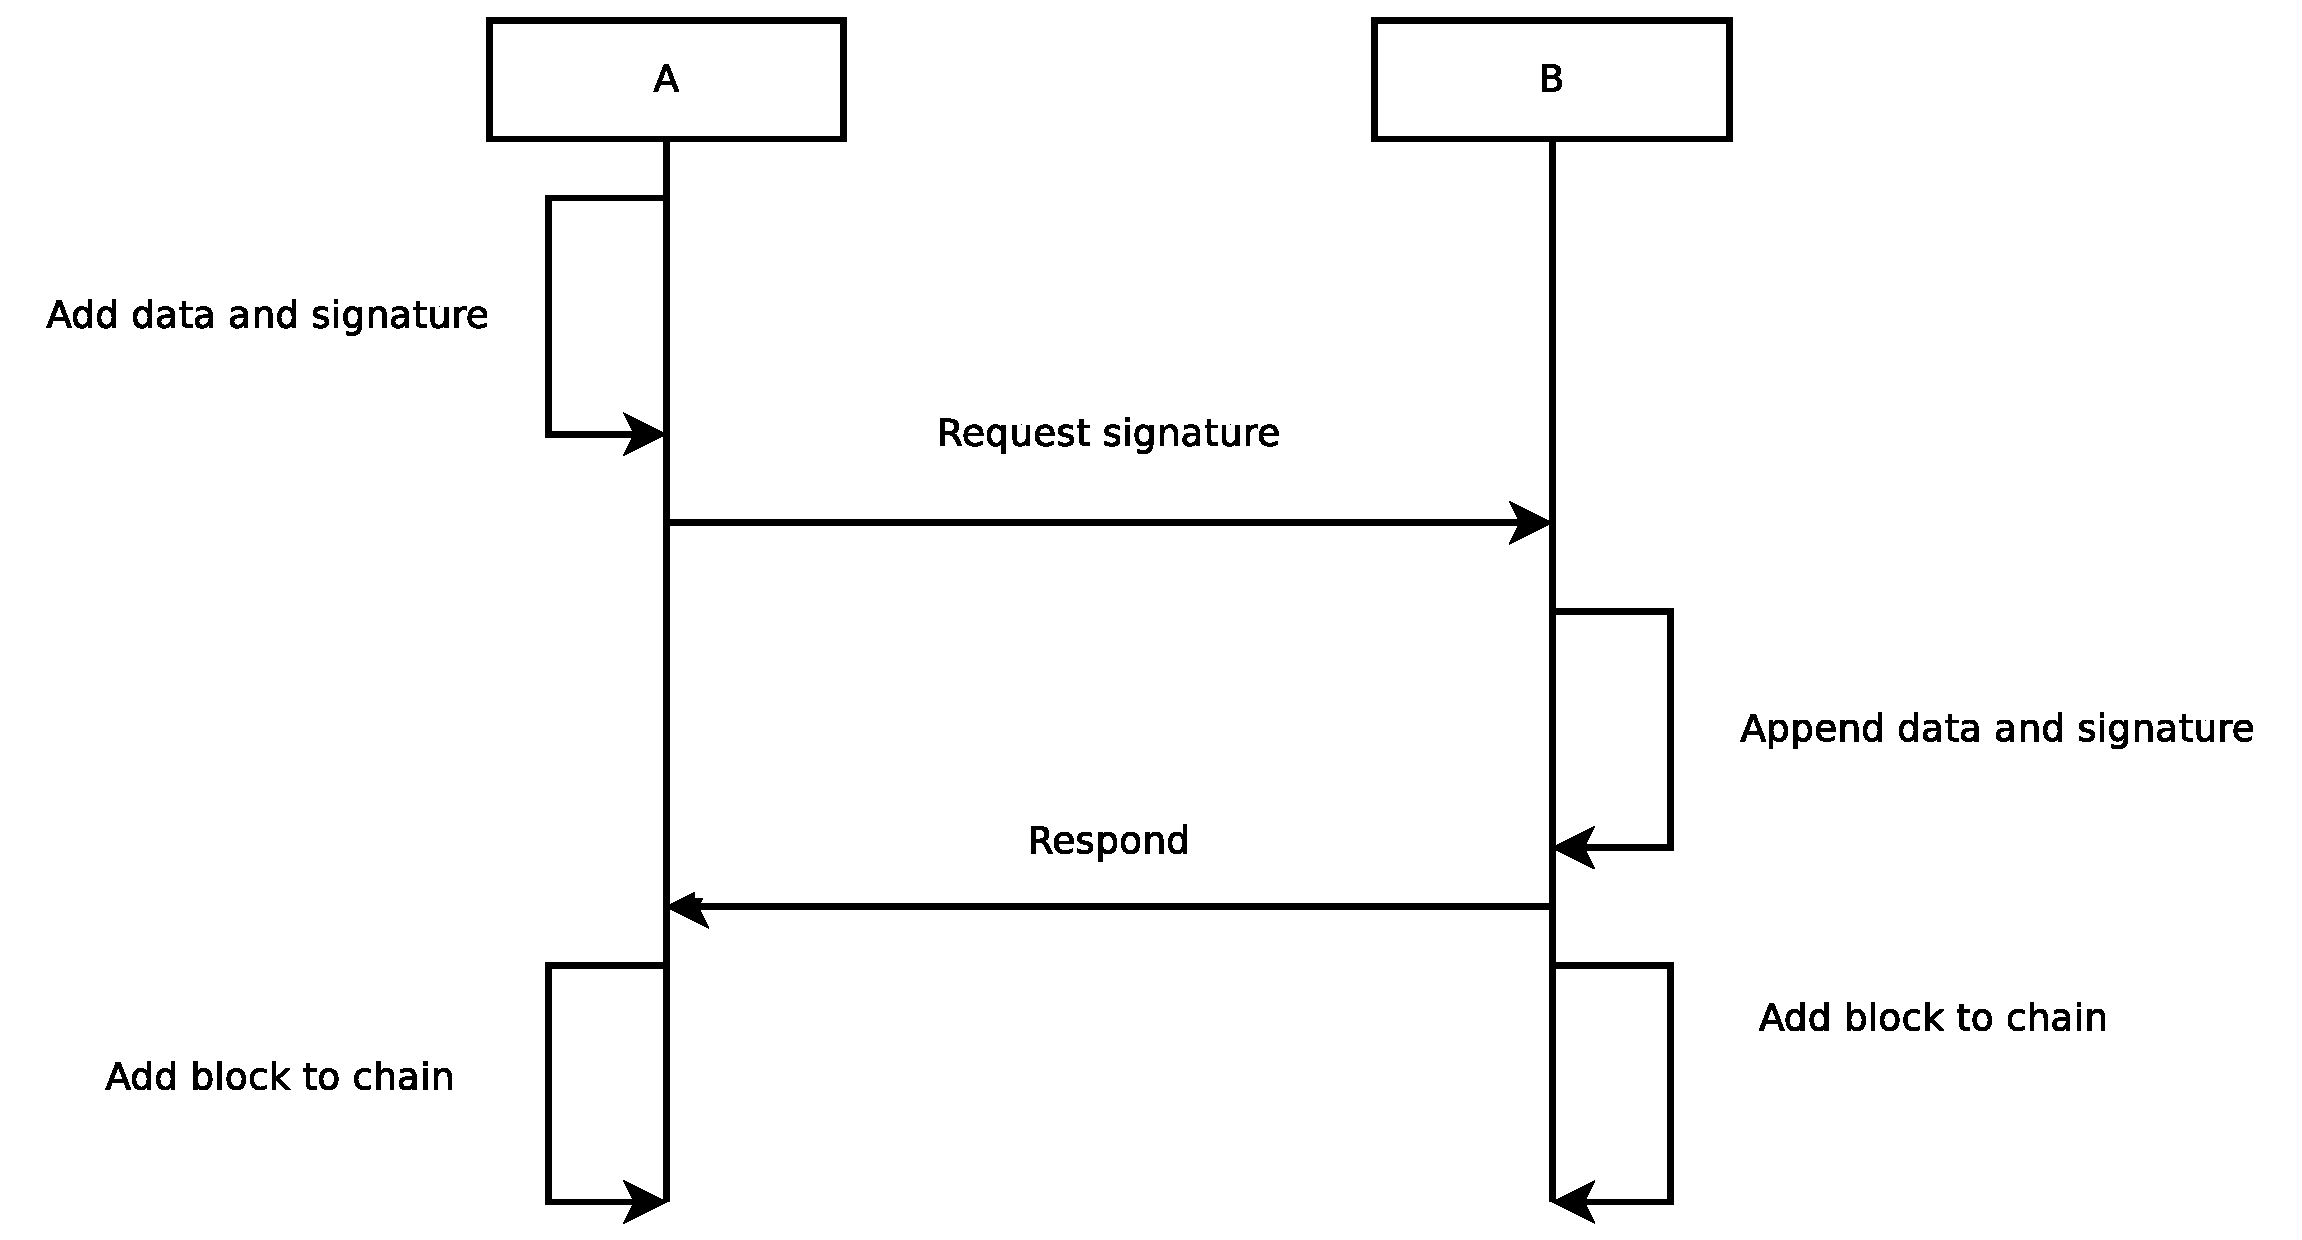
\includegraphics[scale=0.3]{design/figs/exchange_new.eps}}
\label{fig:exchange-new-sequence}
}

\subfigure[Data added by peer A and B for a new block.]{
	\centerline{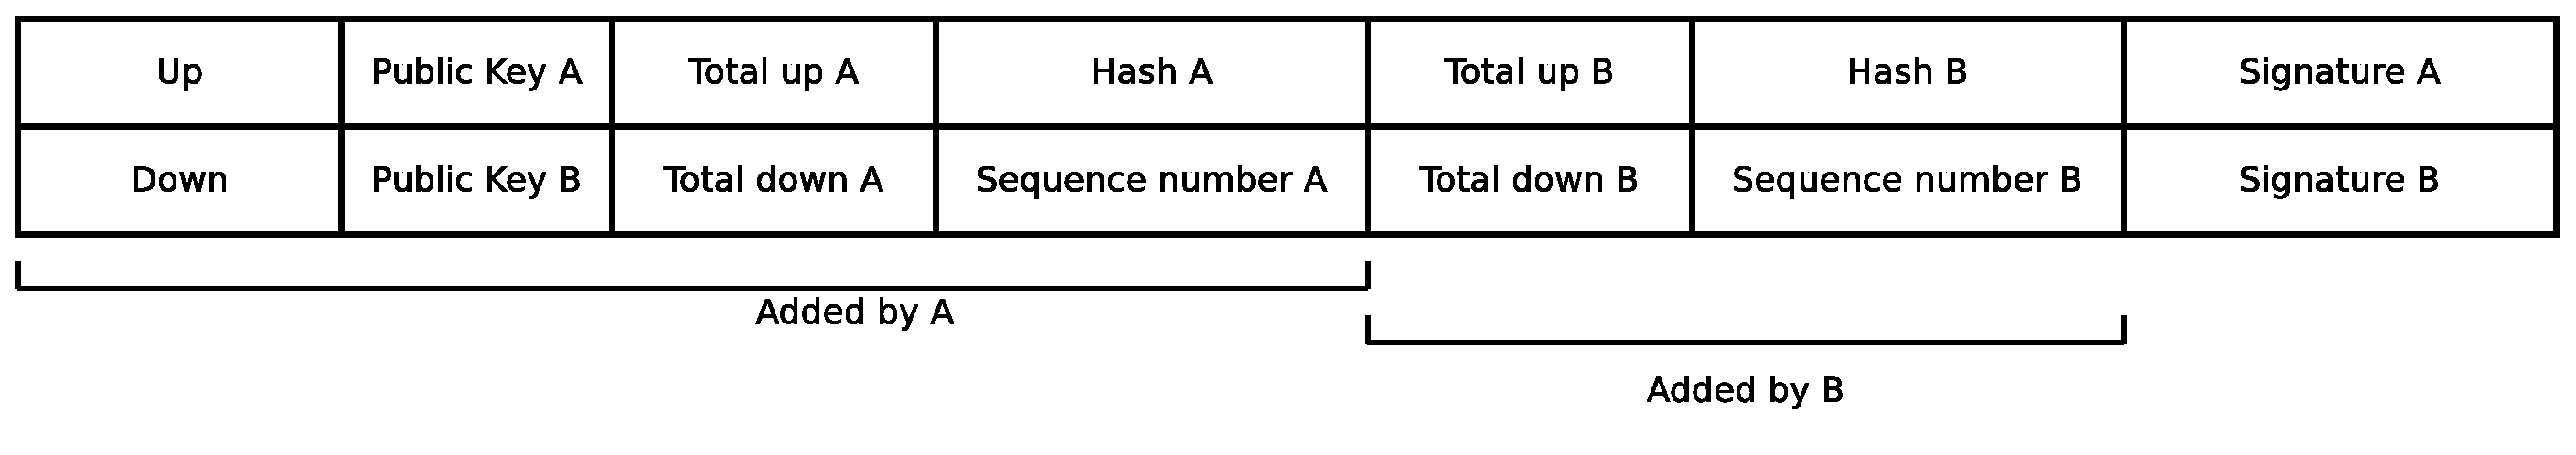
\includegraphics[scale=0.3]{design/figs/packet_creation.eps}}
\label{fig:packet-creation}
}
\caption{Exchanging data for block creation.}
\label{fig:block-creation-new}
\end{figure}

The seeder, A, will create a packet that will be sent to the downloader, B.
A will add to this packet the data uploaded and downloaded data between the peers
that has not yet been added to the MultiChain.
It will add these amounts to its total uploaded and downloaded data
and add these total amounts aswell to the packet.
Finally, it adds the public keys of both peers and its own hash pointer to the packet.
This packet is signed using its private key and sent to the downloader.
The data that A adds can be seen in Figure \ref{fig:packet-creation}.

B will receive this packet and check if the amounts are correct, if the signature is correct,
and if A has not used the previous hash before.
If this is all correct,
then B will add the amounts of uploaded and downloaded data to its own total amounts.
The data contained in the previous packet, the total amounts of B and the hash of the previous block is
inserted into a new packet.
This packet is signed by the private key of B and sent back to A.
The data that B adds can be seen in Figure \ref{fig:packet-creation}.

Both parties now have the data of the block and can add this to their chain and continue forward.
A does this upon receival of the block.
B does this immediatly after sending the return packet to A.
At this point a new block is created.

\subsubsection{Integrating with Dispersy}
\begin{figure}[!h]
\centering
\subfigure[Sequence diagram for block creation.]{
\centerline{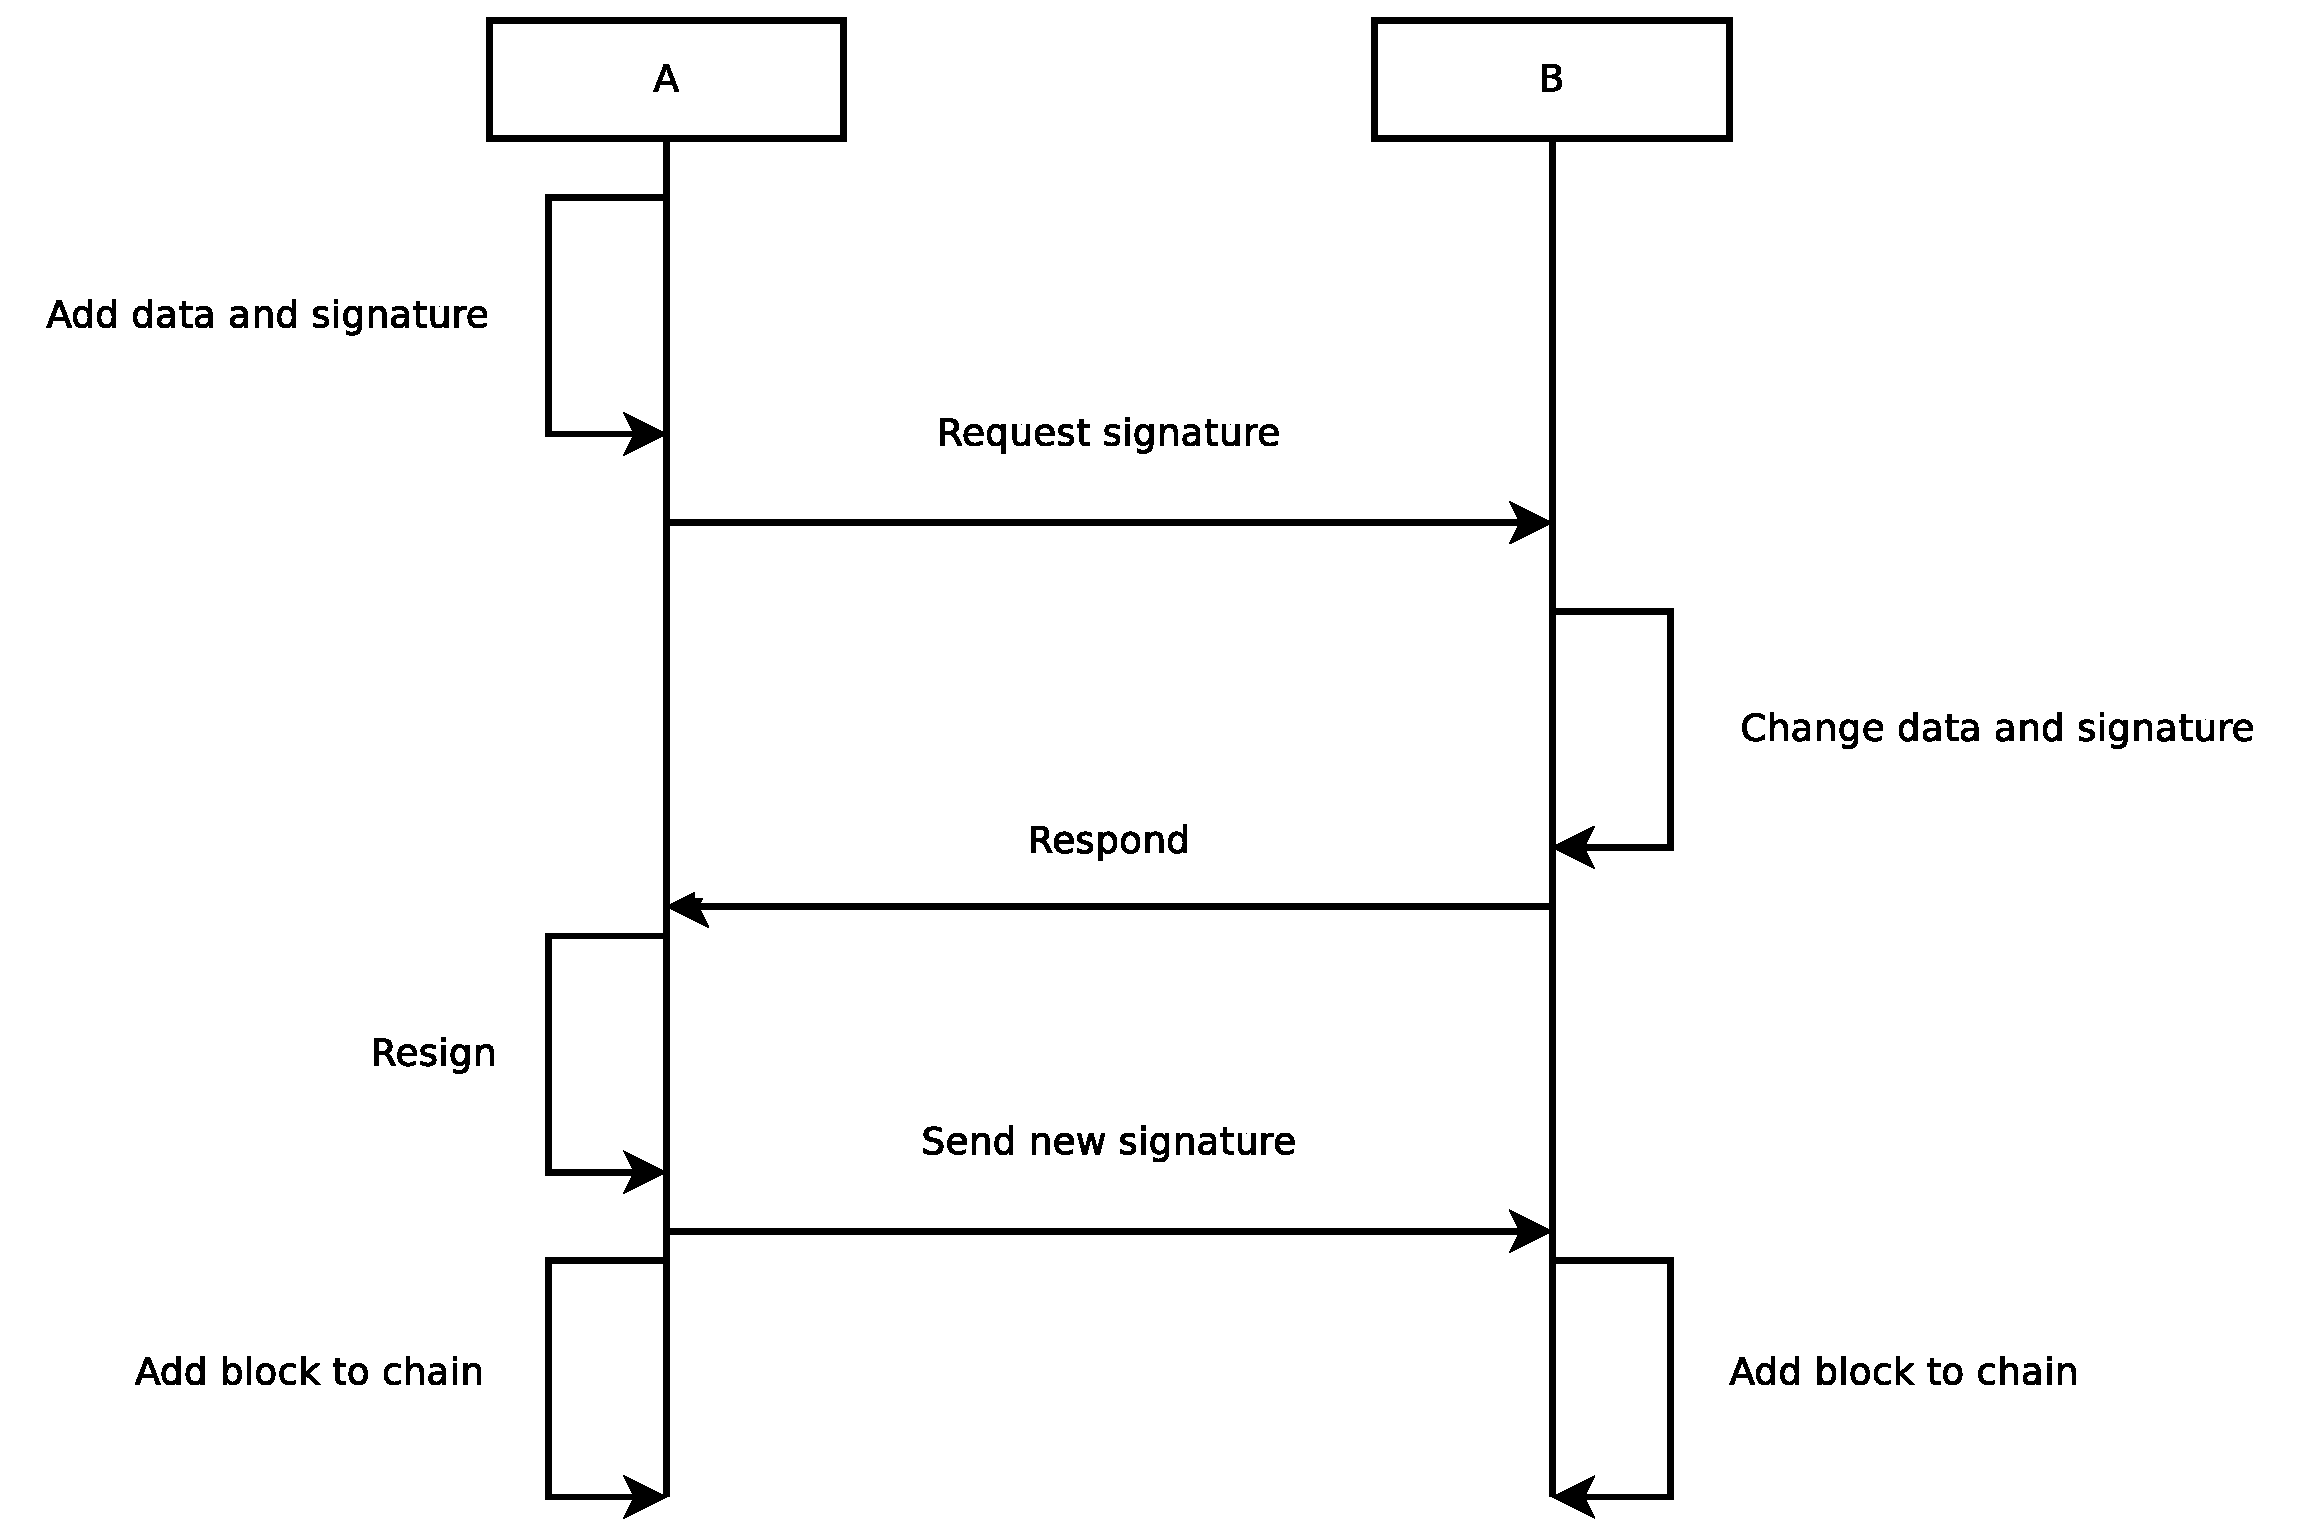
\includegraphics[scale=0.3]{design/figs/exchange_old.eps}}
\label{fig:exchange-old-sequence}
}

\subfigure[Data added by peer A and B for a new block.]{
	\centerline{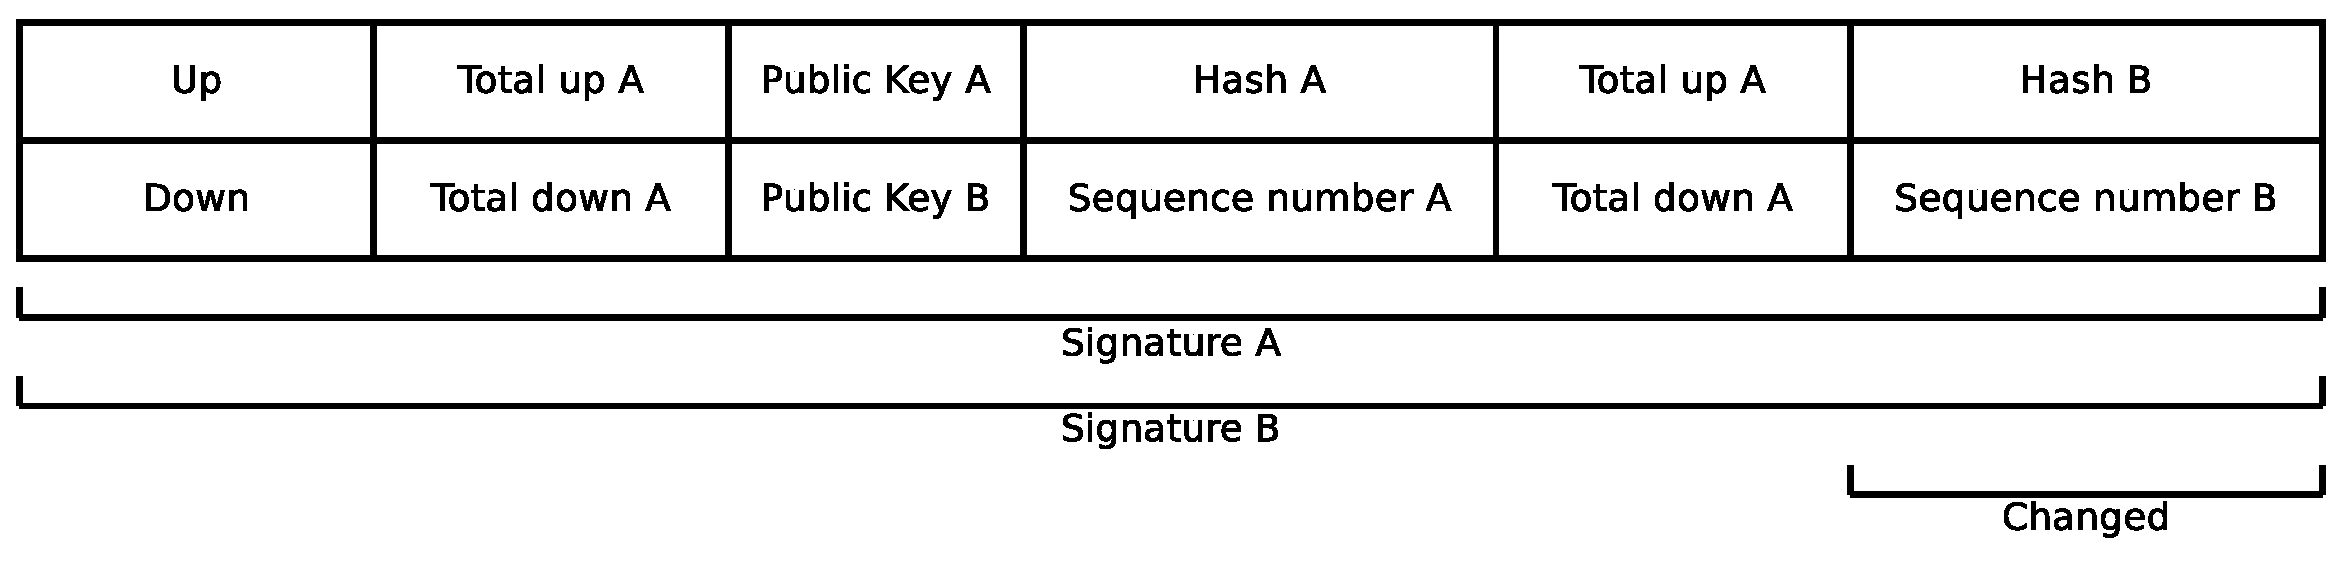
\includegraphics[scale=0.3]{design/figs/signature_old.eps}}
    \label{fig:payload-signature-old}
}
\caption{Exchanging data for block creation using existing functionality.}
\label{fig:block-creation-old}
\end{figure}
Within Dispersy functionality was already build to create a message, sign the message
and request multiple nodes to also provide their signature on this message.
This existing functionality could be used by MultiChain to exchange signatures
between A and B for the creation of a new block.

A would initiate a message, insert its data into this message, sign the message, and send this message to B.
The functionality would allow B to accept the message and provide its signature or
modify the message and then provide its signature.
Only B knows the hash of its head node, and the total up and total download metrics.
So B will always modify the message and insert its own data in the message.
But this would invalidate the signature of A,
because the signature of A was also placed on the empty part of the message where the data of B is inserted.
The contents of the message and who signs what can be seen in Figure \ref{fig:payload-signature-old}.

After B returns the message,
A would have to resign the message.
But B also needs this valid signature from A before it can add the block to its own chain.
So A would need to send a third message to with the new, valid signature back to B.
A sequence diagram can be seen in Figure \ref{fig:exchange-old-sequence} of how it would work in Dispersy.
Functionality was added to Dispersy that allows to append data in a signature request.
This allows the full signature exchange to be achieved within two messages.
\section{Block persistence}
The blocks in the chain have to be persisted to be usable over a prolonged time.
A persistence layer is added to the MultiChain community
that provides all functionality to persist blocks and query blocks.
This layer extends and uses functionality of the Database class in Dispersy.
An overview of the layering in the software architecture can be seen in Figure \ref{fig:persistence-layer}.

\begin{figure}
	\centerline{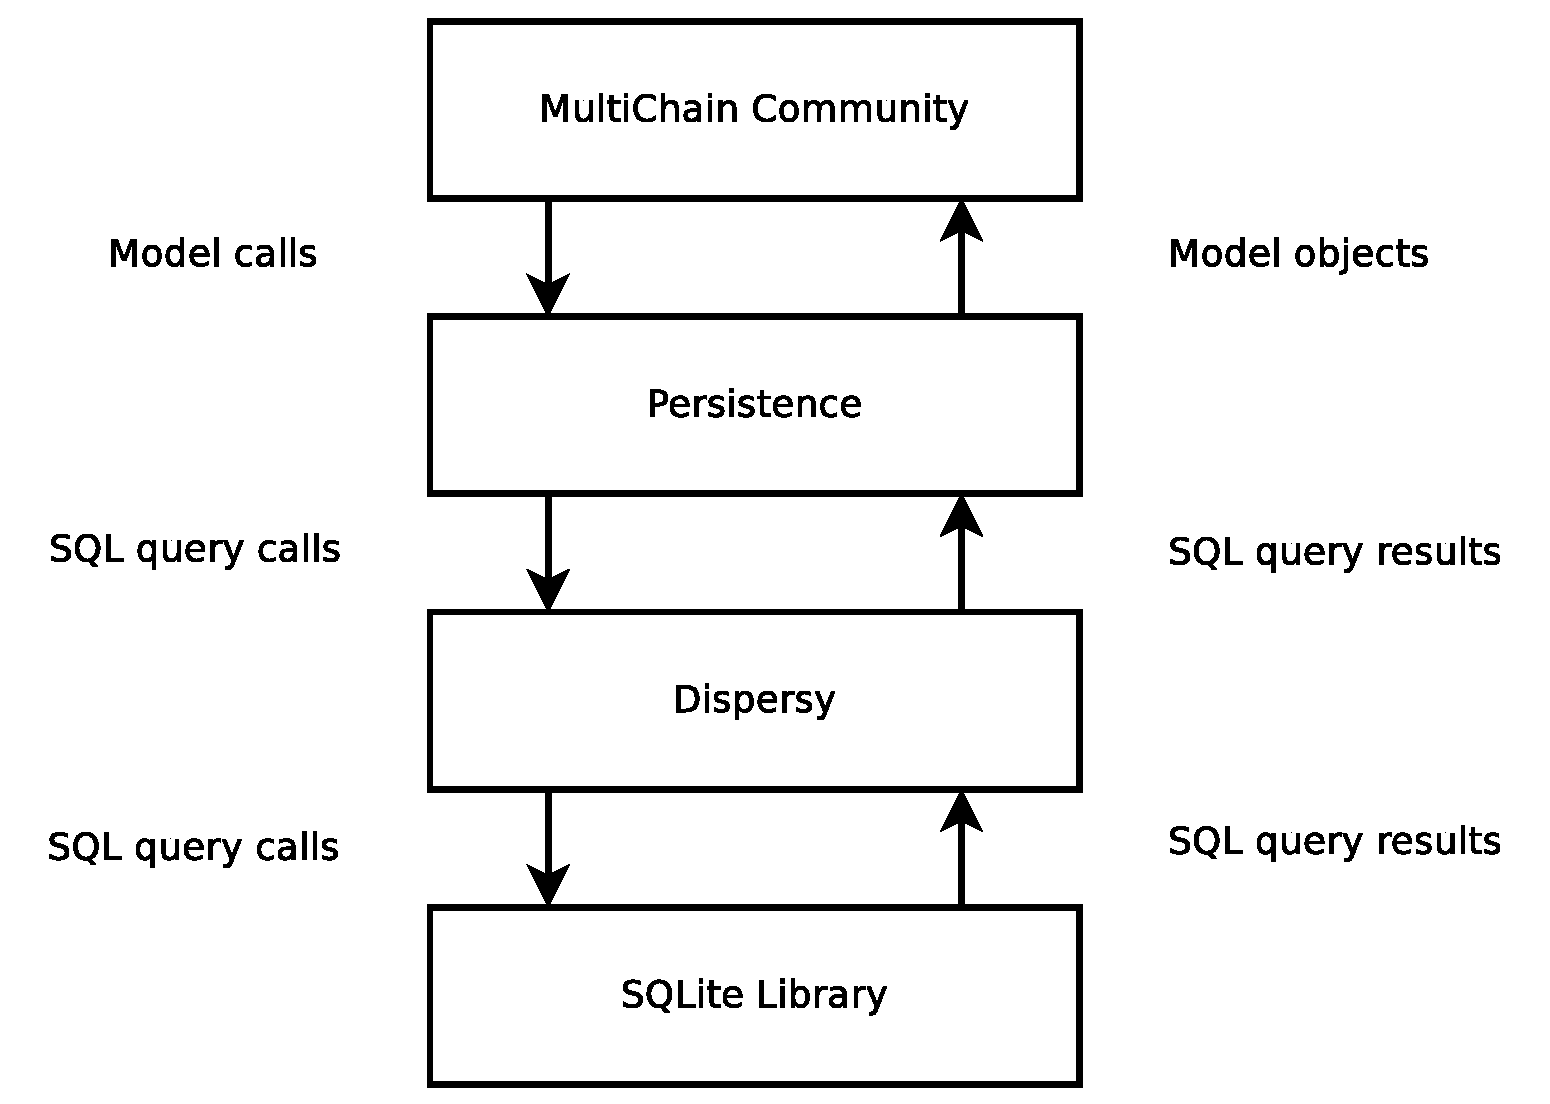
\includegraphics[scale=0.3]{design/figs/persistence-layer.eps}}
	\caption{Persistence layering in the software architecture}
	\label{fig:persistence-layer}
\end{figure}

The MultiChain Community calls functions in the persistence layer that have implicit knowledge about the model.
The Persistence layer formats SQL queries and passes these to the Dispersy layer.
The Dispersy layer performs several sanitation checks and passes these queries to the SQLite Library.
The SQLite Library and Dispersy layer both return the result of the SQL query.
These results are transformed by the Persistence layer into objects of the model usable by the MultiChain Community.

The only information that is saved are blocks.
The information all fits within one table.
A single block is saved as a single record called a row in a relation database.
Every attribute of a block is a single column in the row.
All attributes are saved directly into the database,
except for the public keys.
These public keys are hashed and these hashes are used as an identifier, called mid, in Dispersy.
The public keys are already saved in the Dispersy database.
When a block is retrieved from the database the public key is retrieved from Dispersy using the mid.

Every attribute is queryable in the database.
A public key can be converted to mid and is searched this way.
Every attribute is queryable to make the system  extensible
and usable when the next incremental steps are implemented.
It is presently unknown what information precisly will be needed,
so every information is now made available for the future.

\subsection{Dispersy database}
Dispersy keeps track of information on its own.
A record is kept of any message that can be retrieved using a message id.
The message is saved in a converted format and will be decoded when the message is retrieved.

Instead of storing information in a separate database,
the information could have been retrieved from the Dispersy database.
But the Dispersy database is not queryable.
Because all the information is stored in a converted format
that prevents queries to search the message for its contents.
For this reason, the dispersy database is not used and a separate database is used.

A future, possible improvement to Dispersy would be to save messages queryable in its database.
This would eliminate the current need for separate databases that contain aggregrated information.
The information is stored in two places within Tribler and this could be eliminated.
It would reduce the disk footprint and the amount of read/write transactions
as only one database would have to be maintained.
The I/O ineractions are a problem according to Tribler maintainers.

\section{Irrevocable proof-of-help}
Digital signatures have the property to be non-repudiable of origin \cite{VanderLubbe-crypto}.
After signing a message the signer cannot later deny providing his signature.
Only in the possesion of a secret key can a signature be made,
so only the signer could have made the signature.
This is assuming the secret key was not comprimised.

This property results in that after creating a block
both participants can no longer deny involvement in that block.
Because they cannot repudiate their own signature
The blocks become durable records aand are irrevokable and irrefutable.

\section{Publicly known free-riding}
The system will make a node's share ratio publicly accessibly,
but it will expose and limit freeriding in several other ways.

The window of potential freeriding is chosen by the willingness of seeders to be altruistic.
The creation of blocks is driven by seeders,
downloaders cannot postpone creation of blocks and continue freeriding.
If downloaders do not participate in block creation,
then uploading to them will stop.

A created block will force a downloader to expose his own freeloading,
because he will have to add his own total amount of uploaded data and total amount of downloaded data.
If he has not contributed his share and only downloaded,
then his total downloaded data will be much higher then his total up.
His freeloading is exposed as a result.

Downloaders cannot repudiate downloading.
For they granted their signature to a block containing information about the amount that they downloaded.
A freerider cannot try to hide his freeriding afterwards.

\section{Crawler}
We implemented a crawler that visits other nodes and request the full chain of that node.
The crawler was built to be used for the experiments and
is a first step in a more sophisticated crawler that will help to solve the known vulnerabilities.
These vulnerabilities will be described in chapter \ref{problems}.

\subsection{Recursively request blocks}
Dispersy provides a list of other nodes that were recently found
and can report when the node itself is found by another node.
Both are sources of destinations nodes that the crawler will visit
and request the chain from.

The crawler will first request from a node the block with sequence number $-1$.
This denotes that he wants the latest block in his chain.
The node returns this block to the crawler.
The crawler will persist the block if it is not yet know.

The newly retrieved block is chained to two blocks with the previous hashes.
The crawler will check if these blocks are present in the database.
If any block is not present,
then the crawler will request that particulair block.
The peer, to whom the block belongs to, has to be known in Dispersy.
If the peer is not known, the block is ignored.
This is done recursively untill the crawler reaches the genesis block of the chain.
In this fashion a breadth first search is implemented for any unknown block
that is present in the chain before the latest block.

The crawl tries to aggregrate as much blocks as possible.
But it gives no certainty that the full MultiChain is collected.
The crawler is able to crawl a disconnected MultiChain,
if for every disconnected partition a peer is known by Dispersy.

\begin{figure}
	\centerline{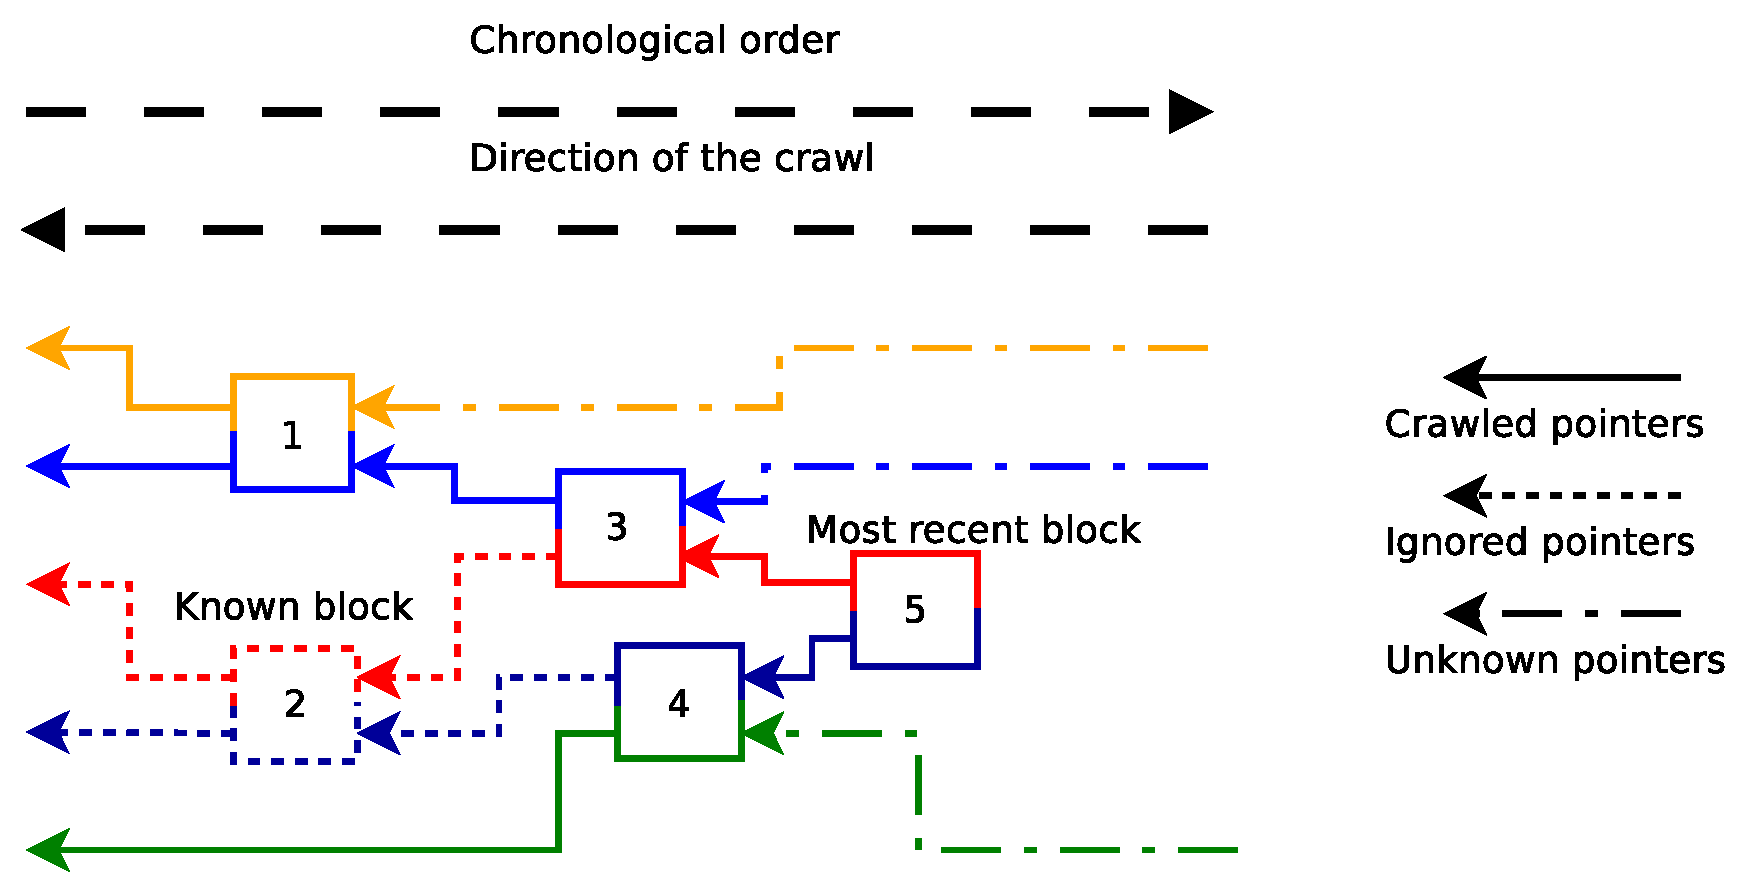
\includegraphics[scale=0.3]{design/figs/crawler-version2.eps}}
	\caption{Example of the crawler looking for unknown blocks. The crawler retrieves the most recent block and crawls older blocks.}
	\label{fig:crawler-example}
\end{figure}

An example can be seen in Figure \ref{fig:crawler-example}.
In this example the line arrows denote paths that the crawler follows,
dotted lines are paths that the crawler ignores,
half dotted lines are paths that the crawler will not know about.
Block 2 is already known by the crawler.
Block 5 is retrieved first by the crawler and the crawler sees hash links to block 3 and 4.
These are retrieved and the block finds links to block 1 and 2.
Because block 2 is already known, it is ignored.
Only block 1 is retrieved.
The crawler continues to follow the links further outside the displayed example.
The half dotted lines are not know by the crawler untill a block is retrieved that contains these paths.
The crawler will retrieve these blocks if for example the most recent block is requested.

\subsection{Recreation over retransmission}
An effort was made to try to reuse code of the community for the crawler and to not introduce another payload type in the community.
The attempt would reuse payload classes and authentication classes already used in the community for the creation of blocks.
This effort failed, because Dispersy cannot handle recreation of messages well
and would invalidate blocks that were recreated.

As said before, Dispersy also keeps tracks of messages received.
The messages containing a block requested by the crawler could be retrieved and retransmissioned forward
instead of being retrieved from the MultiChain database itself.
This would eliminate the need to construct a message and encode the message before it could be send,
because the encoded format is saved and can be retrieved and send immediately.
This was not used as it would be impossible to distinguish messages received as an response to a signature request or a crawler request.
The two types of responses cannot be processed in the same way.
A response to a signature requests has to influence the way a node responds to interactions
and a crawler response should not.

In the end, the crawler uses recreation of a block from the local database and uses a new payload type to forward blocks.
The main reasons this implementation was chosen is
that implemenation was very simple and had none of the above mentioned problems.
Maintainabillity is also much easier this way
as different types of messages are not using the same functions to be received in the code.
This might not be known by a new programmer working with the code.

\subsection{Improvements}
The crawler is a first, simple step towards a more sophisticated crawler.
Tribler has implemented already more sophisticated crawlers for Bartercast
and these techniques can be reused for the MultiChain crawler.
For example bloom filters can be used in conjunction with the knowledge
that every record is a part of the chain to quickly request multiple blocks\cite{broder-bloomfilter}\cite{logiotatidis-splash}.
Blocks could also be send in a more efficient way by sending multiple blocks per message.
Secondly, blocks that belong to a different node than the crawled node are requested,
but the location of this different node is only known by chance.
Dispersy only keeps track of 20 peers at any time, so the chance is low that the node is among these nodes.
The chance can be improved by asking if the first contacted node knows the location of the different node.



